\documentclass [a4paper,11pt] {report}
\usepackage{graphicx}
\usepackage{pdfpages}
\usepackage{fancybox}
\usepackage[francais]{babel}
\usepackage[utf8]{inputenc}
\usepackage[T1]{fontenc}
\usepackage{amsmath,amsfonts,amssymb}
\usepackage{fancyhdr}
\usepackage{stackrel}
\usepackage{xspace}
\usepackage{url}
\newcommand{\dsp}{\displaystyle}

\setlength{\parindent}{0pt}
\setlength{\parskip}{1ex}
\setlength{\textwidth}{17cm}
\setlength{\textheight}{24cm}
\setlength{\oddsidemargin}{-.7cm}
\setlength{\evensidemargin}{-.7cm}
\setlength{\topmargin}{-.5in}


%%%%%%
% Pour mise-en-forme des fichiers Ada
%
% voir exemple en fin de ce fichier.
%
% ATTENTION, requiert encoding utf-8 (voir 2ième "\lstset" ci-dessous)
 
\usepackage{listings}
\lstset{
  morekeywords={abort,abs,accept,access,all,and,array,at,begin,body,
      case,constant,declare,delay,delta,digits,do,else,elsif,end,entry,
      exception,exit,for,function,generic,goto,if,in,is,limited,loop,
      mod,new,not,null,of,or,others,out,package,pragma,private,
      procedure,raise,range,record,rem,renames,return,reverse,select,
      separate,subtype,task,terminate,then,type,use,when,while,with,
      xor,abstract,aliased,protected,requeue,tagged,until},
  sensitive=f,
  morecomment=[l]--,
  morestring=[d]",
  showstringspaces=false,
  basicstyle=\small\ttfamily,
  keywordstyle=\bf\small,
  commentstyle=\itshape,
  stringstyle=\sf,
  extendedchars=true,
  columns=[c]fixed
}

% CI-DESSOUS: conversion des caractères accentués UTF-8 
% en caractères TeX dans les listings...
\lstset{
  literate=%
  {À}{{\`A}}1 {Â}{{\^A}}1 {Ç}{{\c{C}}}1%
  {à}{{\`a}}1 {â}{{\^a}}1 {ç}{{\c{c}}}1%
  {É}{{\'E}}1 {È}{{\`E}}1 {Ê}{{\^E}}1 {Ë}{{\"E}}1% 
  {é}{{\'e}}1 {è}{{\`e}}1 {ê}{{\^e}}1 {ë}{{\"e}}1%
  {Ï}{{\"I}}1 {Î}{{\^I}}1 {Ô}{{\^O}}1%
  {ï}{{\"i}}1 {î}{{\^i}}1 {ô}{{\^o}}1%
  {Ù}{{\`U}}1 {Û}{{\^U}}1 {Ü}{{\"U}}1%
  {ù}{{\`u}}1 {û}{{\^u}}1 {ü}{{\"u}}1%
}



\title {{ {\huge Rapport du projet}} \\
``{\em Décomposition en polygones monotones}'' }

\author {Equipe 82 \\
PIERUCCI Dimitri \\ GOUTTEFARDE Léo}
\date{Vendredi 10 Avril 2015}
% \date{Vendredi 10 Avril 2015\endgraf\bigskip
% Equipe NN}

\lhead{Projet d'Algorithmique 2}
\rhead{Rapport}

\begin{document}
\pagestyle{fancy}
\maketitle

\begin{center}
\section* {Introduction }
\end{center}

Nous avons réalisé l'intégralité du sujet, dont pour commencer la conception d'un package d'arbre binaire de recherche générique, que nous avons décidé d'implémenter à l'aider d'un AVL pour optimiser au maximum l'efficacité, ce qui permet ainsi à toutes les opérations demandées (insertion, suppression, recherche) de s'effectuer en $O(log_2(n))$.

L'exécutable décompose sans problème les polygones au format .in en polygones monotones, et effectue également des mises à l'échelle et translations lors de l'export en code \textit{svg} afin d'obtenir des polygones qui ne débordent pas des dimensions de la figure.

De plus nous avons bien respecté la contrainte de coût au pire cas de $O(h)$ pour l'écriture des fonctions \lstinline!Noeuds_Voisins! et \lstinline!Compte_Position!, en intégrant notamment l'actualisation du champ \lstinline!Compte! des noeuds de l'AVL au sein des opérations de rotation et autres.

Finalement les libérations mémoire sont bien effectuées et il n'y a pas de memory leak.


$\newline$

%Choix / pq
\section* {1\hspace{5mm}Choix d'implémentation }

\subsection* {1.1\hspace{3mm} Structures de données}

L'essentiel de nos structures de données est défini au sein du fichier common.ads :

\begin{lstlisting}
type SimplePoint is record
        X : Float := 0.0;
        Y : Float := 0.0;
end record;

type Segment is array (Positive range 1 .. 2) of SimplePoint;
package Segment_Lists is new Ada.Containers.Doubly_Linked_Lists ( Segment );


type Point is record
        Pt : SimplePoint;
        InSegs : Segment_Lists.List;
        OutSegs : Segment_Lists.List;
end record;

package Point_Lists is new Ada.Containers.Doubly_Linked_Lists ( Point, "=" );
package Point_Sorting is new Point_Lists.Generic_Sorting( "<" );
\end{lstlisting}


Nous avons choisi d'utiliser une première structure \lstinline!SimplePoint! de représentation des points simples, et une seconde \lstinline!Point! composée d'un \lstinline!SimplePoint! ainsi que des deux listes de segments respectivement entrants et sortants.

Les segments sont quant à eux représentés à l'aide d'un tableau de deux \lstinline!SimplePoint!.

Pour finir nous avons utilisé les listes chaînées fournies par la bibliothèque standard Ada afin de parcourir les points et segments simplement. Aussi, le tri des points de gauche à droite est ainsi réalisé grâce aux package de tri générique des listes.



\subsection* {1.2\hspace{3mm} Organisation du code}

Nous avons créé un package \lstinline!Parseur! pour implémenter le parseur des fichiers .in, un package \lstinline!SVG! chargé des affichages en \textit{svg}, un package \lstinline!Decompose! implémentant la majorité des fonctions de décomposition en polygones monotones, et pour finir un package \lstinline!AVL! chargé de la gestion des arbres binaires de recherche équilibrés.

Le programme principal est implémenté au sein du fichier main.adb, qui est relativement simple.

Pour finir, nous avons également réimplémenté la majorité des comparaisons entre flottants afin de les réaliser correctement à $\epsilon = 0.0001$ près.


\section* {2\hspace{5mm}Tests }

\subsection* {2.1\hspace{3mm} Tests unitaires}

Nous avons bien évidemment testé le code au fur et à mesure tout au long du projet, tout particulièrement le package \lstinline!AVL! ainsi que la fonction de comparaison des segments essentielle à son bon fonctionnement.

Pour ces tests nous avons principalement utilisé les fichiers test\_avl.adb et test\_comp.adb.

\begin{center}
  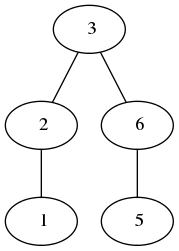
\includegraphics[scale=0.5]{entiers.png}
\end{center}

Le fichier test\_avl.adb implémente l'exemple d'arbre d'entiers du sujet afin de vérifier les valeurs attendues et en exporte un fichier \textit{test\_avl.dot}, ce qui donne la figure ci-dessus après export en png via le logiciel dot.


En effet nous avons réalisé une fonction d'export générique \textit{dot}, \lstinline!AVL.Generic_Display.Export!, afin de vérifier le bon équilibrage des arbres et visualiser les problèmes de comparaison de segments.
Cette fonction d'export permet notamment de visualiser la valeur des clefs (entiers, segments) facilement.


Le fichier test\_comp quant à lui, parse certains fichiers de test afin d'en extraire certains segments problématiques et en vérifier la bonne comparaison, indiquant la qualité de la comparaison des segments.




\subsection* {2.2\hspace{3mm} Mesures de performance}

L'exécutable est relativement rapide et décompose les polygones de test 1 à 8 en 3 à 5 millièmes de seconde.


\end{document}


